\subsubsection{Elección de motores} \mbox{} \vspace{10pt} \\
El sistema de locomoción es el responsable de la traslación del robot. Las configuraciones más comunes son las siguientes: diferencial, sincrónico, triciclo, ackerman y omnidireccional.

Como nosotros tomamos como base la estructura ya definida para el robot Hermes III, adoptamos el sistema mecánico de locomoción omnidireccional, el cual permite mayor libertad de movimiento que los sistemas de ruedas clásicos, Los robots que implementan este sistema pueden moverse en cualquier dirección sobre el plano y en cualquier momento sin la necesidad de hacer movimientos previos para modificar su trayectoria. Requiere ruedas que permitan movimientos en más de una dirección. Este sistema puede ser implementado con tres o cuatro ruedas.

Las ruedas omnidireccionales ruedan en el sentido de avance, pero, también se pueden desplazar lateralmente con gran facilidad como se observa en la siguiente figura:

Los actuadores tienen por misión generar el movimiento de los elementos del robot según las órdenes dadas por la unidad de control. De manera general, los actuadores utilizados en robótica pueden emplear energía neumática, hidráulica o eléctrica.

Las características de control, sencillez y precisión de los accionamientos han hecho que los actuadores eléctricos sean los más usados. Dentro de los actuadores eléctricos pueden distinguirse tres tipos diferentes:

Motores de corriente continua (DC):
\begin{itemize}
   \item Controlados por inducción
   \item Controlados por excitación
\end{itemize}

Motores de corriente alterna (AC):
\begin{itemize}
   \item Síncronos
   \item Asíncronos
\end{itemize}

Se opta por motores de corriente continua, como el que se muestra en la figura siguiente, pues el torque generado es proporcional a la diferencia de potencial aplicado a los terminales de alimentación y el sentido de giro depende de la polaridad, facilitando de este manera el control.

Este tipo de motores pequeños y de bajo costo generalmente presentan como inconveniente que no publican sus curvas. Para resolver este inconveniente se realizaron distintos experimentos. Esencialmente se construyó un montaje que consta de una polea con un peso conocido, que no es más que un recipiente con agua como muestra la siguiente figura, la polea se fija al eje del motor para realizar los experimentos.

Se realizaron distintas corridas variando la tensión y corriente, se tomaron mediciones de velocidad y torque. Con estos datos se construyeron las curvas de rpm-torque y corriente-torque, como se muestra la siguiente tabla:

\begin{center} \begin{tabular}{|c|c|c|}
   \hline
       Tensión & Velocidad & Torque \\
   \hline
       3V & 25 RPM & 0,3 Kg*cm\\
   \hline
       6V & 67 RPM & 1 Kg*cm\\
   \hline
       12V & 96 RPM & 2 Kg*cm\\
   \hline
\end{tabular} \end{center}

Con estos experimentos, también, se midió la respuesta del sistema a un escalón.

\begin{figure}[H]
    \centering
    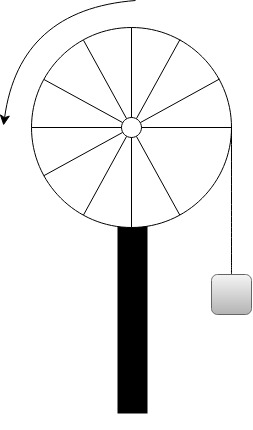
\includegraphics[width=0.25\linewidth]{images/medicion_rpm.jpg}
    \caption{Montaje para medir el torque}
    \label{fig:medicion_torque}
\end{figure}

Para la alimentación de los motores es necesario un circuito integrado especial que permite manipular de manera segura la corriente eléctrica de los motores y a su vez brinde la posibilidad de controlar la polaridad de los bornes donde se conectan los mismos para cambiar su sentido de giro.

Esta solución se ofrece en el mercado en el integrado comúnmente denominado "Driver Dual para Motores L298N", también conocido como "puente H", el cual posee a su vez un regulador de voltaje LM7805 para alimentar la parte lógica del integrado L298N.

El sentido de giro de un motor estará definido por dos pines cuyos valores establecerán la polaridad de los terminales de alimentación del motor respectivamente. Existen dos pares de pines por cada motor.

Para el control de estos integrados vamos a usar cuatro canales PWM del microcontrolador ESP-32, los cuales van a establecer el sentido de giro y fuerza del motor.